\documentclass[12pt]{report}
\usepackage[a4paper, margin=1in]{geometry}
\usepackage{graphicx}
\usepackage{amsmath}
\usepackage{hyperref}
\usepackage{setspace}
\usepackage{natbib} % for bibliography
\usepackage{titlesec} % to customize section spacing
\usepackage{cleveref}

% Algorithm package
\usepackage{algorithm}
\usepackage{algpseudocode}
\setstretch{1.5}

% Reduce spacing between sections
\titlespacing*{\section}{0pt}{0.5em}{0.5em} % [left, before, after]
\titlespacing*{\subsection}{0pt}{0.5em}{0.5em}
\titlespacing*{\subsubsection}{0pt}{0.5em}{0.5em}

% Reduce space between items in itemize
\usepackage{enumitem}
\setlist[itemize]{topsep=0pt, itemsep=0pt, partopsep=0pt, parsep=0pt}

\begin{document}
\sloppy
\begin{titlepage}
    \centering
    % Title
    \vspace*{1.5in}
    {\Huge\bfseries Term Paper Report\\[1.5em]}
    % Course Information
    {\large \textbf{Course Name:} \textit{Advances in Operating Systems Design}}\\[0.5em]
    {\large \textbf{Course Code:} \textit{CS60038}}\\
    \vspace{1in}
    % Author Information
    {\large \textbf{Submitted By:}}\\[1em]
    {\large Bratin Mondal\\\textbf{Roll No.:} 21CS10016}\\[1em]
    {\large Datta Ksheeraj\\\textbf{Roll No.:} 21CS30037}\\
    \vspace{1in}
    % Institution Details
    {\large Department of Computer Science and Engineering}\\[0.5em]
    {\large Indian Institute of Technology Kharagpur}\\
    \vfill
    % Date of Submission
    {\large \textbf{Date of Submission:} \today}
\end{titlepage}

\begin{abstract}
This term paper explores two advanced technologies in the field of data management and storage: Facebook's Tectonic Filesystem and Google's Monarch. The Tectonic Filesystem is engineered for efficiency at exascale, designed to manage vast amounts of data with exceptional performance and reliability. In contrast, Monarch serves as a globally distributed, highly available time-series database, supporting many of Google's critical applications by enabling low-latency queries and efficient storage of telemetry and monitoring data at an unparalleled scale.

For both technologies, we first examine the motivation behind their design, followed by an analysis of their technical and practical aspects. Finally, we provide our evaluation and insights based on a critical assessment of the respective papers.
\end{abstract}

\tableofcontents
\newpage

\chapter{Facebook's Tectonic Filesystem: Efficiency from Exascale}

\section{Introduction}

\subsection{Overview: What is Tectonic?}\label{sec:intro}

Tectonic\cite{tectonic} is Meta's (formerly Facebook) exabyte-scale distributed filesystem, developed to meet the extensive data storage demands of Meta's services. Unlike specialized single-tenant filesystems, Tectonic functions as a general-purpose, multi-tenant solution, capable of serving various types of tenants with diverse data requirements.

A core objective of Tectonic's architecture is to ensure high scalability and efficient resource utilization. Its multi-tenant design enables Meta to consolidate services previously managed in specialized environments, simplifying operations and reducing maintenance costs. Within Tectonic, each tenant can implement specific optimizations, achieving performance levels comparable to custom filesystems while benefiting from shared infrastructure.

Notably, Tectonic is intended solely for Meta's internal services and is not designed for external use. This focus allows Meta to tailor the filesystem to its unique requirements and optimize it specifically for its workloads, without the risks posed by potentially misbehaving external tenants, aside from unintended issues.

\subsection{Meta's Existing Storage Systems}\label{sec:existing}

Meta's storage infrastructure mainly serves two types of tenants: Blob Storage and Data Warehouse.

\subsubsection{Blob Storage}\label{sec:blob_storage}

Blob Storage is used for large, often unstructured binary data like images, videos, and documents, ranging in size from small files to gigabytes. Blobs require low-latency read and write operations for user-facing applications. Based on access frequency, blobs are categorized into:

\begin{itemize}\label{blob_categories}
    \item \textbf{Hot}: Frequently accessed blobs (e.g., recently uploaded photos).
    \item \textbf{Warm}: Less frequently accessed blobs (e.g., older photos).
\end{itemize}

\subsubsection*{Hot Blob Storage}\label{sec:hot_blob_storage}

Hot blobs were stored in Haystack\cite{haystack}, a distributed system designed to handle large volumes of data efficiently at scale. Haystack employs a flat, key-value model that minimizes metadata storage by storing blob data contiguously, reducing disk I/O and enhancing retrieval performance. With a replication factor of 3, each blob is replicated across three nodes to ensure fault tolerance and high availability. The core design principle is to eliminate unnecessary metadata, as it is not critical for blob storage, thus reducing disk seeks.

\subsubsection*{Issues with Haystack}\label{sec:haystack_issues}
One of the major limitations of Haystack was its high IOPS (Input/Output Operations Per Second) requirements. Originally, Meta's Engineering team designed the system with a replication factor of 3.6, which included 3 for replication and an additional 1.2x for RAID6 redundancy. However, in practice, the devices struggled to meet the IOPS demands, necessitating the addition of more devices to keep up with the load. This issue arose due to advances in disk density, while IOPS capabilities remained relatively unchanged. As a result, the effective replication factor grew to 5.3x, with a significant portion of the storage capacity being underutilized.

\subsubsection*{Warm Blob Storage}\label{sec:warm_blob_storage}
Meta used f4\cite{f4}, a highly efficient distributed filesystem, to store warm blobs. f4 employs Reed-Solomon erasure coding\cite{ReedSolomon1960} for fault tolerance, which enables data redundancy without the significant storage overhead associated with traditional replication. This approach ensures both durability and scalability, making f4 well-suited for large-scale warm blob storage.

\subsubsection*{Issues with f4}\label{sec:f4_issues}
Although f4 proved effective for warm blob storage, the large volume of warm blob data required a significant number of devices. However, the issue arose in that these devices also provided high IOPS capacity, which was unnecessary for the relatively low I/O demands of warm blobs. As a result, a substantial portion of the IOPS capacity remained underutilized, leading to inefficiencies in resource allocation.


\subsubsection{Data Warehouse}\label{sec:data_warehouse}
A Data Warehouse stores structured data, such as user activity logs, social graph snapshots, map-reduce outputs, and other analytics data. It is typically accessed via batch processing jobs with read-heavy workloads, infrequent writes, and less emphasis on latency. Parallel processing models often lead to multiple files in the same directory being read together.

Meta's Data Warehouse storage relied on the Apache Hadoop Distributed File System (HDFS)\cite{hdfs}, which is designed for large file storage across multiple machines. HDFS uses a single NameNode for metadata and multiple DataNodes for file storage, optimized for large files and streaming reads, making it ideal for batch processing workloads.


\subsubsection*{Issues with HDFS}\label{sec:hdfs_issues}
 Capacity of HDFS was constrained by the NameNode's metadata storage, which could not scale to meet Meta's increasing data demands. To address this, Meta's Engineering team partitioned data across multiple HDFS clusters, each with its own NameNode. This solution introduced operational complexity, resembling a 2D-bin packing problem, with one dimension representing data size and the other throughput requirements. The partitioning strategy proved inefficient, requiring manual load balancing across clusters and making system management and scalability challenging. In short, scaling HDFS became an unsustainable solution for Meta's expanding data needs.


\subsection{Design Goals for Tectonic}\label{sec:design_goals}
The limitations of existing storage systems highlighted several key design challenges for Tectonic:
\begin{itemize}\label{design_challenges}
    \item \textbf{Scalability to Exabytes}: Tectonic had to efficiently store and serve massive amounts of metadata to meet Meta's exabyte-scale storage needs.
    \item \textbf{Performance Isolation}: Tectonic needed to ensure performance isolation between tenants, preventing resource contention while also allowing tenants to utilize surplus resources from others.
    \item \textbf{Tenant-Specific Optimizations}: Tectonic had to provide flexibility for tenants to implement custom optimizations typically found in specialized filesystems.
\end{itemize}

\subsection{Existing Solutions}\label{sec:existing_solutions}
Several existing storage solutions have been explored to address similar challenges. Federated HDFS\cite{hadoop_federation} and Windows Azure Storage (WAS)\cite{azure} focus on merging smaller storage clusters into larger ones, utilizing multiple independent namespaces while sharing data nodes. However, this still leads to a bin-packing problem at the namespace level, where it is difficult to determine where to place specific data. Solutions like Ceph\cite{ceph} and Flat Datacenter Storage (FDS)\cite{fds} hash data objects to determine their locations, increasing the range of hash functions to scale. However, this approach requires updating the hash function during each data relocation, which can be highly costly in large-scale systems.


\section{Design of Tectonic}

\subsection{Tectonic Architecture}\label{sec:tectonic_architecture}

A Tectonic cluster is composed of Chunk Stores, Metadata Stores, and Background Services. A Client Library, tailored for various Tectonic use cases, interfaces with the Metadata and Chunk Stores to store and retrieve data. The architecture of Tectonic is illustrated in \Cref{fig:tectonic_architecture}, with additional details provided in the subsequent sections. Tectonic clusters are resilient to host, rack, and power failures at the data center level. For geo-replication, tenants can deploy multiple Tectonic clusters across different data centers.

\begin{figure}[htbp]
    \centering
    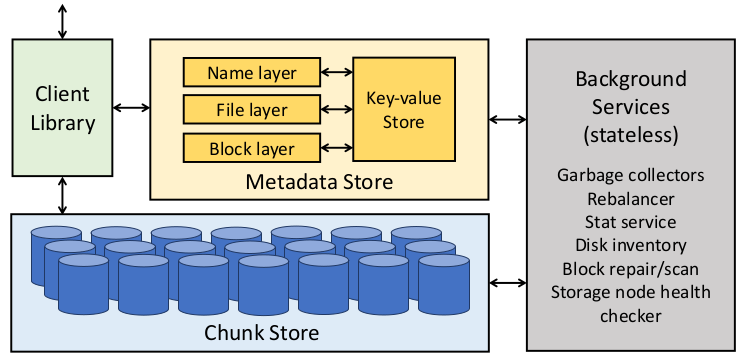
\includegraphics[width=0.8\textwidth]{pics/design.png}
    \caption{Tectonic architecture, with arrows indicating network calls. Filesystem metadata is stored in a key-value store. All components are stateless, except for the Chunk and Metadata Stores.}\label{fig:tectonic_architecture}
\end{figure}

\subsubsection{Chunk Store}\label{sec:chunk_store}
In Tectonic, a file is composed of multiple blocks, each containing several chunks, which are the fundamental data storage unit. The Chunk Store is a flat, distributed object store that manages these chunks and is designed to scale linearly with the number of storage nodes, supporting exabytes of data. This abstraction is managed by the Client Library and the Metadata Store, which handle higher-level abstractions like blocks and files.

Chunks are stored as files on storage nodes, each running a local instance of XFS. These nodes are equipped with 36 hard drives for chunk storage and a 1 TB SSD for XFS metadata and caching frequently accessed chunks. The SSD cache is managed using a flash endurance-aware caching library to optimize performance. Tectonic ensures block durability through Reed-Solomon (RS) encoding or replication. Chunks within blocks are distributed across fault domains for fault tolerance, and background services repair damaged or lost chunks to maintain data durability.

\subsubsection{Metadata Store}\label{sec:metadata_store}
Tectonic addresses the challenge of managing large volumes of metadata by organizing it hierarchically into multiple layers. The Metadata Store is a distributed key-value store, divided into three distinct layers:

\begin{itemize}\label{list:metadata_layers}
    \item \textbf{Name Layer}: Maps directories to the sub-directories and files they contain.
    \item \textbf{File Layer}: Maps files to their associated blocks.
    \item \textbf{Block Layer}: Maps blocks to their corresponding chunks and includes a reverse mapping from chunks to blocks, which aids in garbage collection.
\end{itemize}

Unlike traditional directory mappings where a key maps to a list of values, Tectonic stores keys in an expanded format to enable faster updates. For example, if directory \texttt{A} contains sub-directory \texttt{B} and file \texttt{C}, the keys stored will be \texttt{(A, B)} and \texttt{(A, C)}, rather than a single key \texttt{A} mapping to both \texttt{B} and \texttt{C}. This approach accelerates updates and eliminates the need for locks during the update process. However, listing the contents of a directory requires a prefix scan over the keys.

Another design choice is the use of hash partitioning for the different layers, instead of range partitioning. This method provides better load balancing and helps prevent hotspots in the system, particularly for Data Warehouse parallel processing workloads, as discussed in \Cref{sec:data_warehouse}.

At a lower level, the Metadata Store is powered by ZippyDB \cite{zippydb}, with each node using RocksDB \cite{rocksdb} for storing key-value pairs. Fault tolerance is ensured through replication, utilizing the Paxos consensus protocol \cite{paxos}.

While this design enables scalability and mitigates hotspots, it introduces some challenges. The layered architecture results in increased latency for metadata operations. To address this, Tectonic clients can seal directories, which allows for caching of metadata within the client library. Furthermore, Tectonic does not support atomic cross-directory operations, nor does it provide a direct API for listing the entire contents of a directory. Consequently, clients are required to implement a wrapper around the list API to retrieve the contents of a directory.


\subsubsection{Client Library} \label{sec:client_library}

The Client Library provides a filesystem abstraction using the metadata, operating at the chunk granularity for read and write operations. It enforces \textbf{Single Writer Semantics} by issuing a token when a client opens a file for appending. This token must accompany all subsequent metadata updates, ensuring that only the last process to open the file can perform writes.

For multiple-writer semantics, tenants can implement custom serialization protocols on top of Tectonic. Since the filesystem is intended for internal clients, such protocols are manageable and can be handled by the organization's developers using Tectonic for their specific use cases.


\subsubsection{Background Services} \label{sec:background_services}

Background services ensure consistency, durability, and efficient data management in Tectonic. These services maintain metadata consistency between layers, repair lost data, rebalance storage across nodes, and handle rack drains. They also publish statistics on filesystem usage.

The background services operate on one shard at a time, similar to the Metadata Store. Key services include a garbage collector that cleans up metadata inconsistencies (e.g., caused by failed Client Library operations or lazy object deletion), and a rebalancer and repair service that work together to relocate or delete chunks. The rebalancer identifies chunks needing relocation due to events like hardware failures or increased storage capacity, while the repair service handles the actual data movement, operating on a per-Block layer shard and per-disk basis to scale horizontally. The block layer and the rebalancer service work together to ensure that the total number of copysets\cite{copyset} is maintained, and that chunks are distributed evenly across nodes. 

A copyset refers to a group of replicas of a data chunk stored across different nodes. The system ensures that each chunk of data has multiple copies distributed across multiple nodes to protect against node failures. The copyset concept ensures that even in the event of hardware or network failures, data availability and durability are maintained by limiting the total number of distinct copysets in the system. Each chunk belongs to a specific copyset, and the number of replicas (copysets) is dynamically managed based on system requirements such as redundancy levels, storage capacity, and load balancing.


\subsection{Multitenancy}\label{sec:multitenancy}

Tectonic categorizes resources into two types: \textbf{non-ephemeral} and \textbf{ephemeral}. Non-ephemeral resources change slowly over time and typically do not have dynamic adjustment semantics. An example of this is the storage capacity allocated to a tenant, which is pre-configured and remains static.

In contrast, ephemeral resources change rapidly and require dynamic monitoring and automated adjustments. Examples include storage IOPS capacity and metadata query capacity.

One key challenge is determining the appropriate level at which to manage resources. Providing isolation at the application level is complex due to the difficulty of managing resources across multiple applications. On the other hand, isolation at the tenant level may be too generalized. To address this, Tectonic introduces the concept of \texttt{TrafficGroup} and \texttt{TrafficClass} for managing resources. A \texttt{TrafficGroup} consists of applications with similar storage requirements within a tenant, and each \texttt{TrafficGroup} is assigned a \texttt{TrafficClass}. Tectonic defines three types of \texttt{TrafficClass}: \texttt{Gold} (Latency-sensitive), \texttt{Silver} (Normal), and \texttt{Bronze} (Background services). Tectonic manages resource access both at the global level and per node.

\subsubsection{Global Resource Management}\label{sec:global_resource_management}

The goal of global resource management is twofold: to limit resource usage and to efficiently share surplus resources across tenants. To achieve this, Tectonic employs a modified version of the leaky bucket algorithm, utilizing high-performance, near-real-time distributed counters.

The resource management process works as follows:

\begin{itemize}\label{list:resource_management}
    \item A resource counter is incremented for the corresponding \texttt{TrafficGroup} whenever a resource is used.
    \item If spare capacity is available, it is allocated for use.
    \item If a tenant exceeds its allocated capacity, the system checks for surplus capacity within other \texttt{TrafficGroups} of the same tenant.
    \item If no surplus capacity is found, the system then checks for spare capacity in other tenants.
\end{itemize}

When sharing resources between \texttt{TrafficGroups}, the request is treated as the \texttt{TrafficClass} of the lower-priority group. For example, if a \texttt{Gold} \texttt{TrafficGroup} requests resources from a \texttt{Silver} \texttt{TrafficGroup}, the request is treated as \texttt{Silver}. This prevents excessive increases in high-priority traffic, ensuring that the system remains stable and that many \texttt{Gold} requests can still meet their requirements.

\subsubsection{Per-Node Resource Management}\label{sec:per_node_resource_management}

The aim of per-node resource management is to prevent hotspots and ensure that the latency requirements for high-priority traffic, such as \texttt{Gold} class traffic, are met.

To achieve this, a Weighted Round-Robin (WRR) scheduling approach is employed. In this scheme, a request is skipped if its quota has already been used or if granting it would exceed the quota.

Several optimizations are applied to improve resource utilization:

\begin{itemize}
    \item Lower-priority request classes can yield their turn to higher-priority requests if there will still be enough time to service the lower-priority requests afterward.
    \item The number of non-\texttt{Gold} traffic requests in the queue for a disk is limited if there are pending \texttt{Gold} requests.
    \item Disks may rearrange requests to prioritize higher-priority traffic. If a \texttt{Gold} request is pending for a certain threshold amount of time, non-\texttt{Gold} requests may be deferred to prioritize the \texttt{Gold} request.
\end{itemize}

It is important to note that resource sharing at the node level is unnecessary, as it has already been handled globally.

\subsubsection{Access Control}\label{sec:access_control}

Tectonic employs a token-based access control mechanism to ensure that only authorized clients can access the system. In this system, each layer generates a token that must be included in subsequent requests to the next layer. The token is piggybacked on the request-reply. This mechanism effectively controls access by verifying the presence of a valid token in each request.

\subsection{Tenant-Specific Optimizations}\label{sec:tenant_specific_optimizations}

As mentioned in \Cref{sec:client_library}, the client library communicates directly with the chunk stores at the chunk granularity. This approach enables the optimization of read and write operations for specific tenants.

\subsubsection{Data Warehouse Write Optimizations}\label{sec:data_warehouse_optimization}

Data Warehouse storage has read after complete write semantics that is data is only read after the write operation is complete. This allows for optimizations such as: 

\subsubsection*{Asynchronous Writes}\label{sec:asynchronous_writes}

To optimize write operations, applications buffer writes until enough data is accumulated to form a block of the desired size. RS-Encoding is then done at the client itself, reducing the amount of data that needs to be transmitted to different nodes. This approach also reduces the number of network calls and disk seeks, enhancing write performance.

Importantly, there is no inconsistency introduced because metadata is only updated after the complete write operation has been successfully finished. This approach guarantees that data consistency is maintained throughout the write process.

\subsubsection*{Hedged Quorum Writes}

Hedged quorum writes aim to improve write latency by sending reservation requests to more nodes than the minimum required for a successful operation. Rather than waiting for the write to complete on all nodes, the system only waits until a majority of blocks have been successfully written, at which point the client is notified. 

This method effectively reduces the 99th percentile latency, enhancing the system's responsiveness and providing faster acknowledgment to clients.

\subsubsection{Blob Storage Optimizations}\label{sec:blob_storage_optimization}

\subsubsection*{Consistent Partial Block Appends}

To optimize append operations in blob storage, the system ensures that appends are consistent by waiting until the quorum size of appends is reached. This ensures data integrity and reduces unnecessary writes. Additionally, only the block creator is allowed to perform append operations, maintaining consistency and preventing data corruption.

Once an append operation is completed, the metadata is updated with the post-append block size and its corresponding checksum, ensuring consistency and reliability in the storage system.

\subsubsection*{Reencoding Blocks for Storage Efficiency}

Reencoding blocks for storage efficiency is made possible by the Client Library-driven design. Unlike traditional file systems, which typically require preconfiguration for file storage, this design allows more flexibility in optimizing storage. Specifically, blocks are reencoded from replicated formats to Reed-Solomon (RS) after a certain amount of time has passed. This process reduces the storage overhead associated with replication, enhancing storage efficiency and reducing costs.


\section{Tectonic in Production}

Meta's Tectonic Filesystem supports diverse workloads, including blob storage and data warehousing at exabyte scale. However, certain tenants like Key-Value stores, Deployment Management Systems, and legacy systems don’t use Tectonic due to specialized storage needs. Some services access Tectonic indirectly through major tenants, such as the data warehouse, to avoid the cost of developing individual client libraries. 

\subsection{Exabyte-Scale Multitenant Clusters}

Tectonic is designed for efficient operation at an exabyte scale, supporting diverse workloads under a unified storage system. For example, a typical Tectonic cluster manages approximately 1250 PB of data, representing about 70\% of its capacity, and handles around 10.7 billion files and 15 billion blocks. This scale demonstrates Tectonic's ability to support high-volume, varied workloads effectively.

\subsection{Efficiency from Storage Consolidation}

By consolidating blob storage and data warehouse services, Tectonic enhances resource utilization and manages workload spikes more efficiently. For instance, surplus IOPS from blob storage can be redirected to support bandwidth-intensive spikes from data warehouse workloads. This consolidation reduces the need for separate, overprovisioned systems, optimizing disk usage and lowering overall storage costs.

\subsection{Metadata Management and Load Balancing}

Tectonic manages metadata load spikes efficiently by using load-balancing techniques within its metadata store to maintain high performance. Around 1\% of Name layer shards may hit peak queries per second (QPS) during load surges, but Tectonic handles these spikes with retry mechanisms to sustain responsiveness. Additionally, Tectonic co-designs with the data warehouse to mitigate metadata hotspots from frequent, simultaneous file access. For example, the \texttt{list-files} API provides both file IDs and names, allowing compute engines to distribute file IDs directly to worker nodes, reducing directory query loads on the metadata store.

\subsection{Design Trade-offs}

Tectonic’s design focuses on simplicity and efficiency but involves certain trade-offs.

For \textbf{reconstruction load management}, Tectonic employs contiguous Reed-Solomon (RS) encoding, allowing most reads to be single-disk IO. However, reconstruction reads triggered by failures require higher IO, leading to "reconstruction storms." Tectonic mitigates this by capping reconstructed reads at 10\%, balancing performance with resource usage according to the cluster's workload.

\textbf{Direct access to storage nodes} improves efficiency by avoiding extra network hops, although it adds complexity since Client Library bugs can impact application binaries. Latency-sensitive remote requests are routed through a stateless proxy, optimizing cross-datacenter data access.

\textbf{Metadata latency and partitioning} introduce additional trade-offs. Metadata is stored in a sharded key-value store, which increases latency compared to in-memory storage, prompting optimizations like parallelized file renames. The hash-partitioned design limits recursive directory listing and aggregate space usage queries, which are handled through periodic space aggregation.

These trade-offs enable Tectonic to support scalable, exabyte-level storage while delivering robust performance for diverse workloads.

\medskip

In summary, Tectonic effectively addresses Meta’s large-scale storage requirements through a balance of operational simplicity and resource efficiency, allowing it to replace multiple specialized storage systems and support exabyte-scale, multitenant environments.


\section{Evaluation}

As Tectonic is designed for Meta's internal use, it does not implement many of the semantics required by clients. Instead, it leaves these responsibilities to developers, who are expected to implement them at a higher level while using Tectonic. This design choice allows Tectonic to be more efficient and flexible. However, there are some design choices that are questionable and not explicitly clarified in the paper.

\begin{itemize}
    \item \textbf{Token-based single writer:} The approach of using a token to ensure only one writer can write at a time could lead to deadlock situations if writers alternatively attempt to write to the same file. The paper does not explain how this situation is handled, though it is likely addressed at a higher level by the developers. An alternative could have been to use a lease mechanism, where the writer holds the lease for a fixed time, with forced relinquishment if the lease is not renewed. This would introduce some delay in the event of a writer crash but would be more robust.
    
    \item \textbf{Partial Block Quorum Appends:} The paper describes blob storage tenants waiting for acknowledgment from a quorum of storage nodes, claiming that this provides low latency. However, the handling of writes that are not acknowledged by nodes outside the quorum is not discussed. It is unclear whether this information is stored in the metadata, allowing clients to read only from the nodes within the quorum, or if the client can read some stale data in the interest of low latency. The relaxed consistency model would likely improve performance, but if consistency is a concern, the system should have a mechanism to handle partial writes.

    One option would be to maintain a list of stale chunks of nodes and prevent clients from reading from them. While this would add complexity to the system, it would offer better consistency. It would also allow later writes to be processed even if earlier writes are incomplete at some nodes. This approach would enable clients to send requests to all nodes and wait for a quorum response. However, maintaining an individual list of stale chunks for each node would introduce additional complexity and overhead.

    Another approach would be to serialize writes at each node, maintaining only a list of stale nodes rather than stale chunks. While this avoids the complexity of tracking stale chunks, it would introduce latency since further writes could only proceed on non-stale nodes. This would reduce the effectiveness of partial block quorum appends, as writes would be blocked if any node is stale. This approach would add additional latency to the system.
    
    The exact mechanism used by Tectonic is not described in the paper, so it is unclear how the system handles partial writes and stale data. The paper should have provided more details on this aspect of the system.
\end{itemize}


\chapter{Monarch: Google's Planet-Scale In-Memory Time Series Database}

% \chapter{Introduction}

% \label{Chapter1} % Reference label

% \lhead{Chapter 1. \emph{Introduction}} % Header for each page


\section{Introduction}

Google operates one of the largest and most complex infrastructures in the world, with millions of servers across data centers worldwide. Monitoring and managing performance metrics across this massive infrastructure requires a database capable of handling petabytes of data and millions of queries per second.

Google uses various types of databases, applications each suited for specific tasks. There should be monitoring system over all these systems. Generally a TSDB (Time-Series Database monitoring system is used which captures events along with time stamps)


\subsection{Monarch as TSDB}

A time-series database (TSDB) is a specialized database optimized to handle, store, and analyze time-series data, which consists of data points indexed by time. This type of data typically represents how a system, process, or measurement evolves over time, with each entry or observation paired with a timestamp

At Google, the time-series database (TSDB) landscape has evolved significantly over the years, primarily driven by internal projects and open-source contributions to handle the massive scale of data generated by Google's infrastructure

The initial TSDB developed and used was Borgmon which was replaced with Monarch for reasons discussed later in the report

So currently Monarch is the globally-distributed in-memory time series database monitoring system in Google


% \chapter{The Problem}

% \label{Chapter2} % Reference label

% \lhead{Chapter 2. \emph{The Problem}} % Header for each page

\section{The Problem}

\subsection{Arrival of Borgmon}

\subsubsection{Initial Problem}
Google's infrastructure comprised numerous clusters, each hosting thousands of servers running various applications. The complexity and scale of these clusters made it challenging to monitor system health effectively. Existing monitoring solutions lacked the ability to provide real-time insights into the status of individual servers, services, and applications. This often resulted in:
\begin{itemize}
    \item Need to get a time-based collection of data.
    \item Difficulty in identifying failing or underperforming nodes.
    \item Slow response times to incidents due to limited visibility.
    \item Overwhelming volumes of alerts, many of which were not actionable.
\end{itemize}

\subsubsection{Borgmon Solution\cite{Borgmon}}
Borgmon was designed as a time-series database to provide comprehensive cluster monitoring by implementing:
\begin{itemize}
    \item \textbf{Real-time Monitoring:} Borgmon enabled real-time tracking of system health, resource usage, and performance metrics across all nodes in a cluster.
    \item \textbf{Centralized Data Collection:} It centralized data collection from all servers, allowing for a unified view of the health of the entire infrastructure.
    \item \textbf{Intelligent Alerting:} The system incorporated intelligent alerting mechanisms that reduced noise by prioritizing alerts based on severity and context, thus allowing engineers to focus on critical issues.
\end{itemize}

\subsection{Arrival of Monarch\cite{50652}}

Google shifted from Borgmon to Monarch to address the growing complexity and scale of its monitoring needs, especially as its infrastructure became more distributed and global. Below are the key reasons behind this shift:

\begin{itemize}
    \item \textbf{Scalability and Performance}
    \begin{itemize}
        \item Borgmon was originally designed to monitor Borg, Google’s cluster manager, primarily handling a centralized monitoring model.
        \item As Google’s infrastructure expanded, including global data centers and cloud-based services, Borgmon struggled to scale effectively also making it difficult for engineers to run Borgmon reliably.
        
    \end{itemize}
    

    \item \textbf{Semantic ambiguity}
    \begin{itemize}
        \item Each team created their own Borgmon instance creating their own configuration and variables creating semantic ambiguity
    \end{itemize}

    \item \textbf{No support for Complex Distribution types}
    \begin{itemize}
        \item Some monitoring actually requires complex histograms from which other statistical information is drawn out. This is not supported by Borgmon i.e. We cant store whole of histogram in the records we store
    \end{itemize}
\end{itemize}






% \chapter{Motivation}

% \label{Chapter3} % Reference label

% \lhead{Chapter 3. \emph{Motivation}} % Header for each page

\section{Motivation}

\subsection{Core Solution Ideas}

Keeping in mind the various problems or limitations with Borgmon mentioned in Chapter\ref{Chapter2}, the solutions proposed for each are trivial. This slowly led to the foundation of Monarch, the now widely used replacement of Borgmon.

The solutions for each of the problems were as mentioned below:

\begin{itemize}
    \item \textbf{Scalability and Performance:} The system instead of having a decentralized architecture, now should have a unified one. This now adds on complexity to development of such architecture hence is a good trade off
    
    \item \textbf{Semantic Ambiguity} Simple solution exists for this as we just maintain a uniform rule book all over as we already have a central monarch which we call global monarch
    
    \item \textbf{Complex data types} We have to completely change the record or row which we store as monitoring data. The change in format which we describe in future allows complex distributions such as histogram also to take from the monitored system
    
    \item \textbf{Other Additional Features} Monarch as we shall see have implemented load balancing, data compression which further enables to use the system in a more reliable way. These were also there in Borgmon but its difficult to put up these in a centralised system again
\end{itemize}






% \chapter{Implementation}

% \label{Chapter4} % Reference label

% \lhead{Chapter 4. \emph{Implementation}} % Header for each page

\section{Implementation}

\subsection{Components}

Monarch's architecture includes components categorized by their primary functions: those responsible for storing state, those dedicated to data ingestion, and those focused on query execution.

\begin{figure}[h]
    \centering
    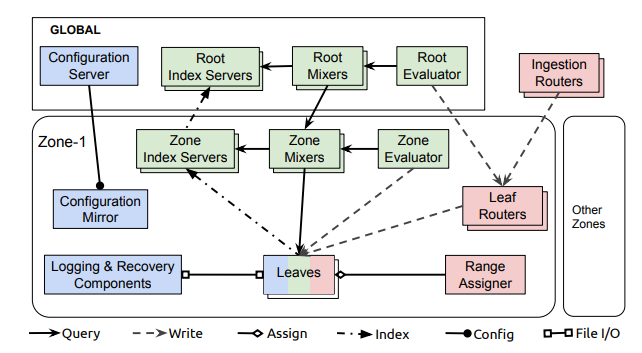
\includegraphics[width=1\textwidth]{pics/monarch.png} % Replace with your image name
    \caption{Overview of Monarch \cite{50652}}
\end{figure}

\subsubsection*{State-Holding Components}

\begin{itemize}
    \item \textbf{Leaves} serve as the primary storage for monitoring data, keeping it in an in-memory time series database.
    \item \textbf{Recovery logs} store monitoring data on disk, mirroring the data held in leaves. Over time, this data is moved into a long-term time series repository.
    \item \textbf{Global configuration server and zonal mirrors} manage configuration data, which is stored in Spanner databases \cite{50652}.
\end{itemize}

\subsubsection*{Data Ingestion Components}

\begin{itemize}
    \item \textbf{Ingestion routers} direct data to leaf routers within the correct Monarch zone, relying on information embedded in time series keys for accurate routing.
    \item \textbf{Leaf routers} receive data bound for a specific zone and forward it to the leaves for storage.
    \item \textbf{Range assigners} handle the distribution of data across leaves, balancing the load within each zone.
\end{itemize}

\subsubsection*{Query Execution Components}

\begin{itemize}
    \item \textbf{Mixers} divide queries into smaller sub-queries routed to and processed by leaves, then combine the results. Queries can be initiated at the root level (handled by root mixers) or at the zone level (handled by zone mixers). Root-level queries require both root and zone mixers.
    \item \textbf{Index servers} provide indexing for each zone and leaf, guiding the distributed execution of queries.
    \item \textbf{Evaluators} periodically execute standing queries (see Section 5.2) by dispatching them to mixers, then write the results back to leaves.
\end{itemize}

\subsection{Data Storage}

Monarch organizes monitoring data into tables that store time series, which are sequences of values recorded over time. Each table includes two main types of columns:

\begin{itemize}
    \item \textbf{Key columns:} These define unique identifiers for each time series, such as the specific machine or service being tracked.
    \item \textbf{Value column:} This stores the historical data points (e.g., memory usage or latency) recorded over time for each time series.
\end{itemize}

Key columns, also referred to as fields, have two sources: targets and metrics.

\subsubsection*{Targets (Monitored Entities)}
\begin{itemize}
    \item A target is the system or component that generates data, like a server, application, or process.
    \item Monarch links each time series to its specific source target, identifying the entity from which the data originates.
    \item Each target follows a schema (template) with specific fields, such as user, job, cluster, or task number for tasks in a computing cluster.
    \item The location field within each target helps Monarch store data near its origin (for instance, data from a specific cluster is stored in the closest zone).
    \item Time series data from the same target are grouped, ensuring related data is stored together and is easier to query.
    \item Target ranges organize targets in alphabetical order to allow efficient data distribution and load balancing, which simplifies group queries.
\end{itemize}

\subsubsection*{Metrics (What We’re Measuring)}
\begin{itemize}
    \item A metric is a specific measurement related to a target, such as the number of requests a server processes or its memory usage.
    \item Each metric has its own schema with particular fields, such as the type of service or command for an RPC request.
    \item Metrics can be various data types, including numbers, strings, or distributions (groups of values that allow for calculations of averages, percentiles, etc.).
\end{itemize}

\subsection{How Data Storage Happens}

The data collection path in Monarch can be broken down into four main steps:

\begin{itemize}
    \item \textbf{Client to Ingestion Router}
    \begin{itemize}
        \item A client application sends time series data to a nearby ingestion router. Monarch's ingestion routers are spread across clusters, allowing data to be gathered close to its origin, thus reducing latency.
        \item Clients frequently utilize Monarch's instrumentation library, which regulates the data write frequency to comply with Monarch's retention policies.
    \end{itemize}
    
    \item \textbf{Ingestion Router to Leaf Router}
    \begin{itemize}
        \item Each ingestion router extracts the location field of the target to determine the appropriate zone for the data, organizing it by geographic or logical regions.
        \item After identifying the target zone, the ingestion router forwards the data to a leaf router within that zone. Zone mappings are dynamically updated.
    \end{itemize}

    \item \textbf{Leaf Router to Leaf Node}
    \begin{itemize}
        \item Within the assigned zone, the leaf router directs data to specific leaf nodes. These leaf nodes manage target ranges, with data sharded lexicographically according to target strings.
        \item Each leaf router keeps an updated range map that indicates which leaf node is responsible for each target range. This map is periodically refreshed by updates from leaf nodes, ensuring uninterrupted data collection even if the range assigner experiences temporary issues.
    \end{itemize}
    
    \item \textbf{Data Storage on Leaf Nodes}
    \begin{itemize}
        \item Upon reaching the assigned leaf node, data is stored in an in-memory time series store and recovery logs. This in-memory store is optimized for efficient handling of timestamp sequences, reducing memory usage.
        \item Data encoding methods, such as \textbf{delta encoding} and \textbf{run-length encoding}, are applied to efficiently manage various time series types, including complex structures like tuples.
    \end{itemize}
\end{itemize}


% \chapter{Organization of Data and Load Balancing}

% \label{Chapter5} % Reference label

% \lhead{Chapter 5. \emph{Organization of data Load Balancing}} % Header for each page

\section{Organization of Data and Load Balancing}

\subsection{Data Organization and Load Balance}

Intra-zone load balancing in Monarch is a strategy used to ensure efficient data storage and distribution across leaf nodes within a zone, minimizing load and optimizing performance. Here’s an in-depth look at how this process works:

\begin{itemize}
    \item \textbf{Schema and Lexicographic Sharding}
    \begin{itemize}
        \item \textbf{Data Organization:} Data is organized in a table schema consisting of a target schema and a metric schema.
        \item \textbf{Sharding by Target:} Only the key columns associated with the target schema are used for sharding data lexicographically. This approach groups all time series for a single target together, which minimizes the ingestion fanout, allowing a single message to carry data for multiple metrics for the same target. As a result:
        \begin{itemize}
            \item Each target's data is only sent to a few (up to three) leaf replicas.
            \item This setup scales the zone horizontally by adding more leaf nodes and simplifies query processing by limiting it to a smaller subset of leaf nodes.
        \end{itemize}
        \item \textbf{Intra-Target Joins:} Common joins between metrics for the same target can be processed within the leaf node, reducing query complexity and making them faster.
    \end{itemize}

    \item \textbf{Replication Flexibility}
    \begin{itemize}
        \item \textbf{Replication Policy:} Monarch allows users to select the number of replicas per target (ranging from 1 to 3), enabling a trade-off between availability and storage cost.
        \item \textbf{Granularity Control:} Users can choose to retain different levels of data detail for each replica, such as retaining only a fine-grained view on one replica and a coarser view on others.
        \item \textbf{Individual Assignment of Replicas:} Each target range replica is assigned independently to avoid overloading a single leaf node, ensuring no leaf node holds multiple replicas of the same range.
        \item \textbf{Distribution Across Failure Domains:} Leaves are distributed across clusters or failure domains. The range assigner ensures replicas of the same range are stored in different domains to enhance fault tolerance.
    \end{itemize}

    \item \textbf{Range Assigner and Load Balancing}
    \begin{itemize}
        \item \textbf{Load Monitoring and Adjustment:} The range assigner actively balances the load by moving, splitting, or merging ranges as needed based on CPU load and memory usage across leaf nodes.
        
    \end{itemize}

    \item \textbf{Ensuring Data Availability}
    \begin{itemize}
        \item \textbf{Simultaneous Data Collection:} During the transfer process, both the source and destination leaves temporarily collect and log data for range $R$ to avoid any data loss and ensure continuous availability.(\textbf{Interesting optimisation})
        \item \textbf{Direct Updates from Leaves:} Leaves keep leaf routers informed about range assignments, rather than relying on the range assigner for updates(\textbf{Interesting optimisation}). This:
        \begin{itemize}
            \item Ensures data integrity, as leaves are the main storage units.
            \item Allows the system to continue working smoothly if the range assigner has a temporary failure.
        \end{itemize}
    \end{itemize}
\end{itemize}



% \chapter{Querying}

% \label{Chapter6} % Reference label

% \lhead{Chapter 6. \emph{Querying}} % Header for each page

\section{Querying}

\subsection{Query Execution}

In Monarch, there are two types of queries:

\textbf{Ad hoc Queries}
These are one-time queries from users outside the system.

\textbf{Standing Queries}
These are periodic queries whose results are stored back in Monarch. Standing queries are used to generate alerts or pre-process data for faster and more cost-effective access later. They can be processed at either the regional zone level or the global root level, based on the type of data and query requirements. Most standing queries are handled at the zone level, making them more efficient and resilient to network issues.

\subsubsection{Query Tree and Execution Levels}
Queries are processed in a three-level hierarchy:
\begin{itemize}
    \item \textbf{Root Mixer:} Receives the query and distributes it to zone mixers.
    \item \textbf{Zone Mixers:} Send the query to relevant leaf nodes based on an index.
    \item \textbf{Leaf Nodes:} Process the data closest to the source.
\end{itemize}
Each query is executed only at the necessary levels, which optimizes processing. The root node checks security, access control, and can rewrite queries for efficiency. Lower levels (leaves and mixers) stream data upwards, where higher levels combine results and manage the flow of data with rate control.

\subsubsection{Replica Resolution}
Data is often replicated, and replicas may vary in quality (e.g., completeness and time coverage). For accurate results, zone mixers resolve which replica is best based on quality criteria and assign target ranges to specific leaves for processing.

\subsubsection{User Isolation}
Monarch is a shared system, so resources are divided among users. Each user’s queries are limited in memory and CPU through cgroups, ensuring fair use.

\subsubsection{Query Pushdown}
Monarch minimizes data transfer by processing as much of the query as possible at the lowest level. This is called “query pushdown” and improves speed by:
\begin{itemize}
    \item Reducing the amount of data transferred to higher levels.
    \item Allowing more concurrent processing.
\end{itemize}
For example, if a query only involves data from one zone, it can be fully processed there without needing root-level involvement. This pushdown approach makes 95\% of standing queries complete within the zone, which also prevents cross-region data traffic and reduces latency.

\subsubsection{Specific Operations at Lower Levels}
Some queries, like \texttt{group by} or \texttt{join}, are pushed to the leaf level when possible, where they process data within the smallest target ranges. For instance, if data for a specific target (like a task) remains within one leaf, that leaf can complete the operation, which reduces work for higher-level nodes.

\subsection{Result Aggregation}
\begin{itemize}
    \item Leaf Nodes process data closest to the source. They handle their assigned "target range" and perform basic filtering and aggregation to reduce data before sending it up.
    \item Zone Mixers gather results from multiple leaf nodes in their region. They combine and further aggregate data, then send only summarized information to the root mixer.
    \item Root Mixer collects data from zone mixers. It completes any remaining aggregation, checks security, and applies final optimizations.
\end{itemize}

% \chapter{My Observations}

% \label{Chapter7} % Reference label

% \lhead{Chapter 7. \emph{My Observations}} % Header for each page

\section{Evaluation}

While Monarch prioritizes high availability and partition tolerance, the trade-off with data consistency could lead to stale reads. This seemed more bold decision to me, instead we should be using better consistency model which does different things based on situation.

For this I thought of implementing a Reinforcement Learning Model which slowly learns the data it handles and performs accordingly.

Also user was given choice to choose the number of replicas and level of granularity. But when scalability is considered and lot of users operate at same time they might over estimate the usage which unnecessarily creates extra load if all created maximum number of replicas.

For this the control given to users must be looked into again, there must be control mechanisms asking users about the data they are going to handle and based on that the system should have some percentage of controlling. Even complete control to the system itself is a waste.



% Bibliography
\bibliographystyle{plain}
\bibliography{references}  % assuming references.bib is the name of your .bib file

\end{document}
